% !TeX root = ../thuthesis-example.tex

\chapter{数据集分析与对比}
\section{开源数据集}
% \subsection{UNSW-NB15}
流量异常检测领域的开源数据集要么过于久远,无法反映当前的网络环境,要么模拟访问环境过于简单,可信度很低。因此流量异常检测领域的高质量的开源数据集很少。本文采用目前应用最为广泛的两个数据集,UNSW-NB15 和 CI-
CDIS2017,尽管这两个数据集也有很多不足。

澳大利亚网络安全中心(ACCS)的网络范围实验室在 KDD99 数据集的基础上,生成了 UNSW-NB15 数据集\cite{moustafa2015unsw} 的原始网络流量数据。UNSW-NB15利用的主要工具是 IXIA PerfectStorm,期望是可以体现网络在实际状况当中所呈现的流量。相比于陈旧的KDD99数据集\cite{ozgur2016review},其更能代表真实的网络流量。

第二个数据集CI-CDIS2017则是由加拿大网络安全研究所(Canadian Institute for Cyber-security)提供。与UNSW-NB15类似,CICIDS2017也是在仿真环境中模拟正常流量和攻击流量生成的。

UNSW-NB15的实验环境划分了3个子网,采用了45个独立的ip地址,持续约30个小时,采集了共100GB的原始网络流量数据。CICIDS2017的实验环境划分了2个子网,分为受害者子网和攻击者子网,受害者子网共有12台主机,攻击者子网共4台主机,累计测量时间持续约5天,共采集了51.1GB的pcap流量数据。由这两者的实验环境可以看出,开源数据集在规模上远远无法和真实流量环境对比。

% 该数据集包括 100GB的.pcap 格式的原始网络流量,具有九种攻击类型,分别是Fuzzers,Analysis,Backdoors,DoS,Exploits,Generic,Reconnaissance,Shellcode和Worms。每种攻击的具体描述和类别数目如表所示。该数据集还包含4个经过特征提取的csv文件,一共2540044 条数据。


% UNSW-NB15 数据集一共包含 47 个特征,其中时间戳,IP 地址,端口号等特征对训练无用,因此有效的特征一共 41 个。 
% 下面对这些特征做一个概括的说明。按照数据集作者的思路,可以分为基本
% 特征,内容特征,时间特征和额外生成的特征这几类。

以UNSW-NB15为例,图\ref{fig:UNSW-NB15数据集生成过程}展示了该数据集的生成过程。首先,通过使用Tcupdump工具监测访问环境中的流量情况,生成pcap文件;然后使用Argus\footnote{https://qosient.com/argus/index.shtml}和Bro-IDS\footnote{https://www.bro.org/index.html}工具从报文信息中直接提取基于数据包和数据流的特征,并根据五元组(源/目的ip地址,源/目的端口号,协议类型)信息进行匹配,此时基本特征、内容特征和时间特征已生成;接下来为了能够更有效地识别攻击,还需要额外生成一些统计特征。最终将这些特征保存成csv文件。



这些数据集生成流程和特征提取方法给后续我们分析清华大学校园网的流量数据提供了参考。


\begin{figure}
    \centering
    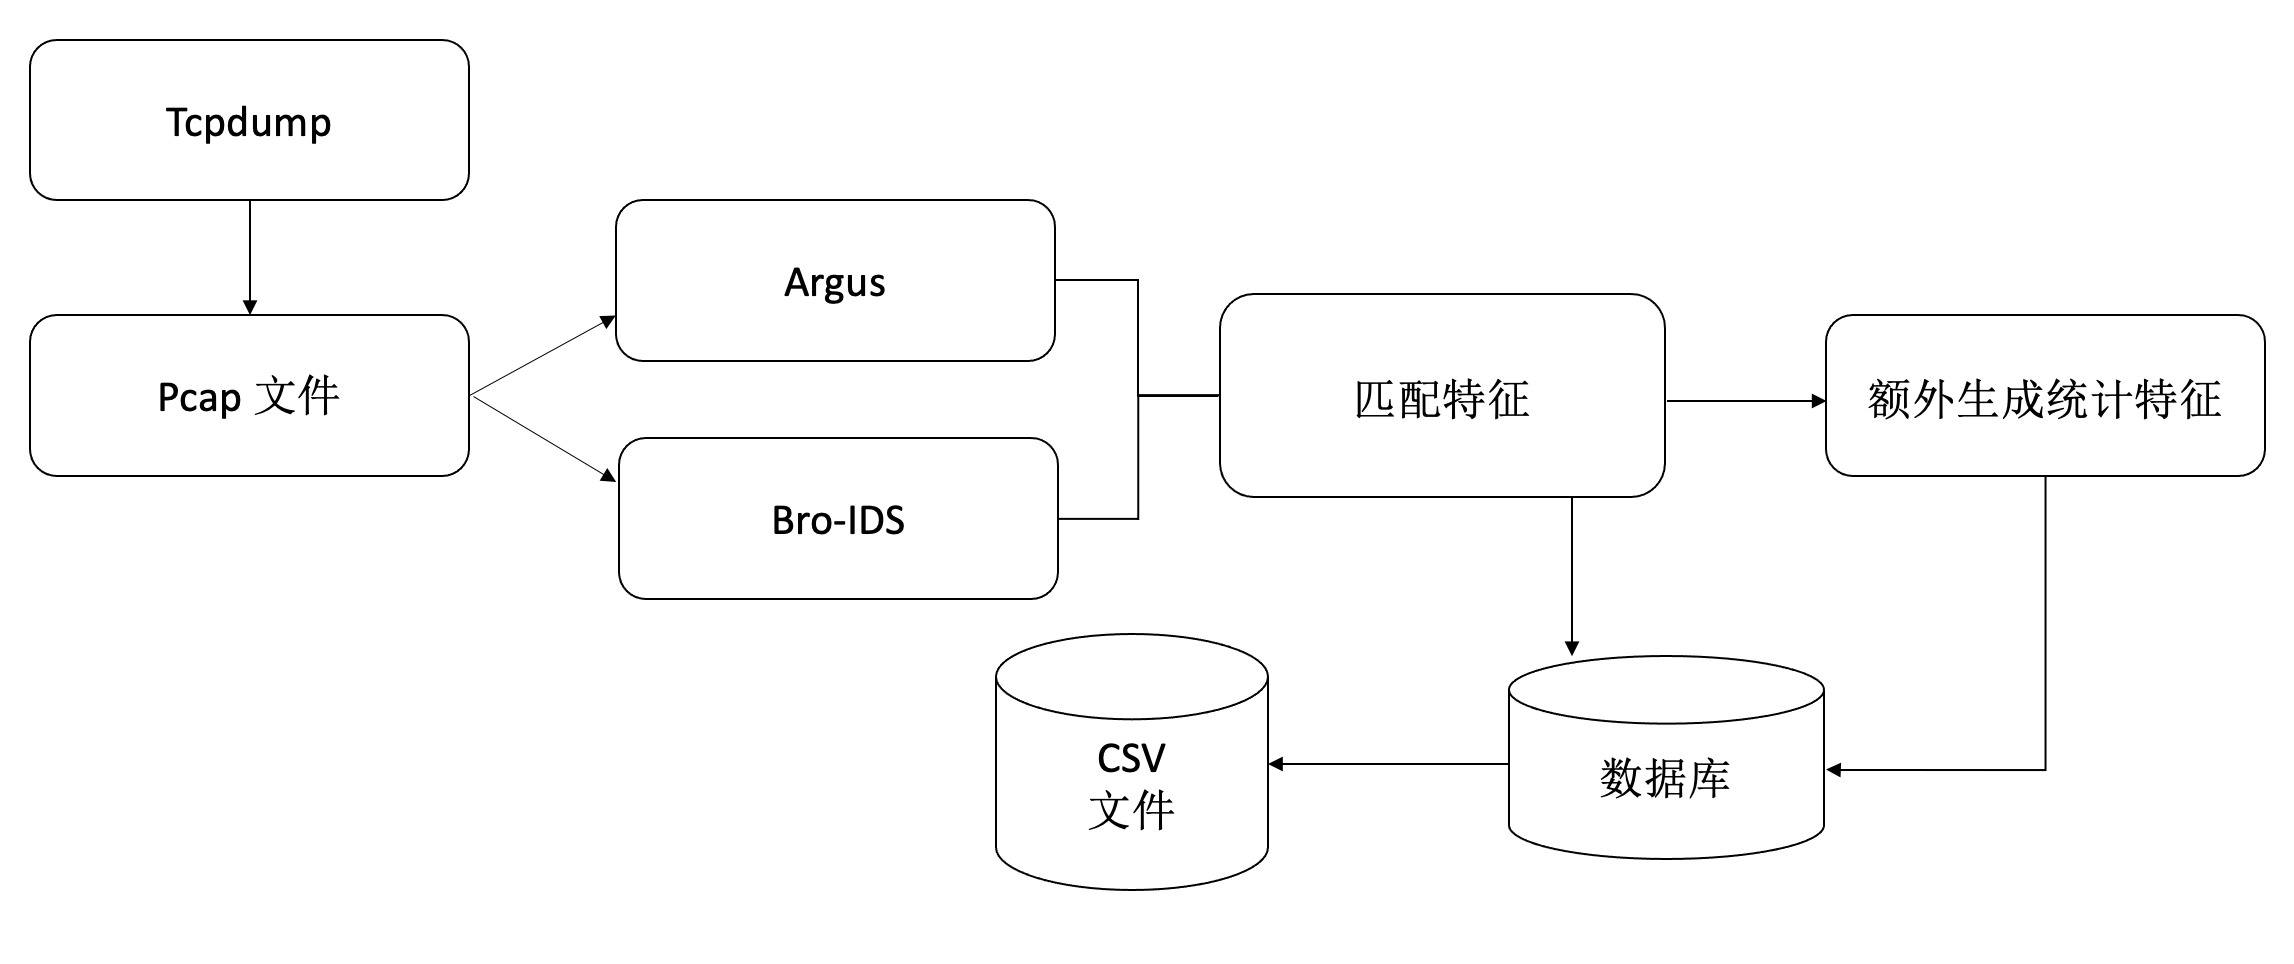
\includegraphics[width=0.6\linewidth]{UNSW-NB15 framework.png}
    \caption{UNSW-NB15数据集生成过程}
    \label{fig:UNSW-NB15数据集生成过程}
  \end{figure}


\section{校园网流量数据集}
清华大学无线网规模巨大,具有超过6万名日活跃用户,13万个可用ip地址,是全球最大的校园无线网之一。通过出口网关的服务器我们可以得到海量的真实流量数据,但是这与可进行分析和训练的数据集之间还有巨大的鸿沟。因此本节参考图\ref{fig:UNSW-NB15数据集生成过程}中的数据集生成流程,结合UNSW-NB15和CICIDS2017两个数据集中特征的特点,生成了校园网的特征数据集。校园网数据集制作流程如图\ref{fig:流量数据集制作流程}所示。首先将pcap流量数据切分成多个会话(session,双向流中所有的数据包),依次从每个会话中提取报文信息以及统计信息构成特征;然后以五元组作为流的标识符,把从SOC平台中得到的告警信息与特征信息合并起来,就生成了最终的数据集。将该数据集命名为CAMPUS数据集。
\begin{figure}
    \centering
    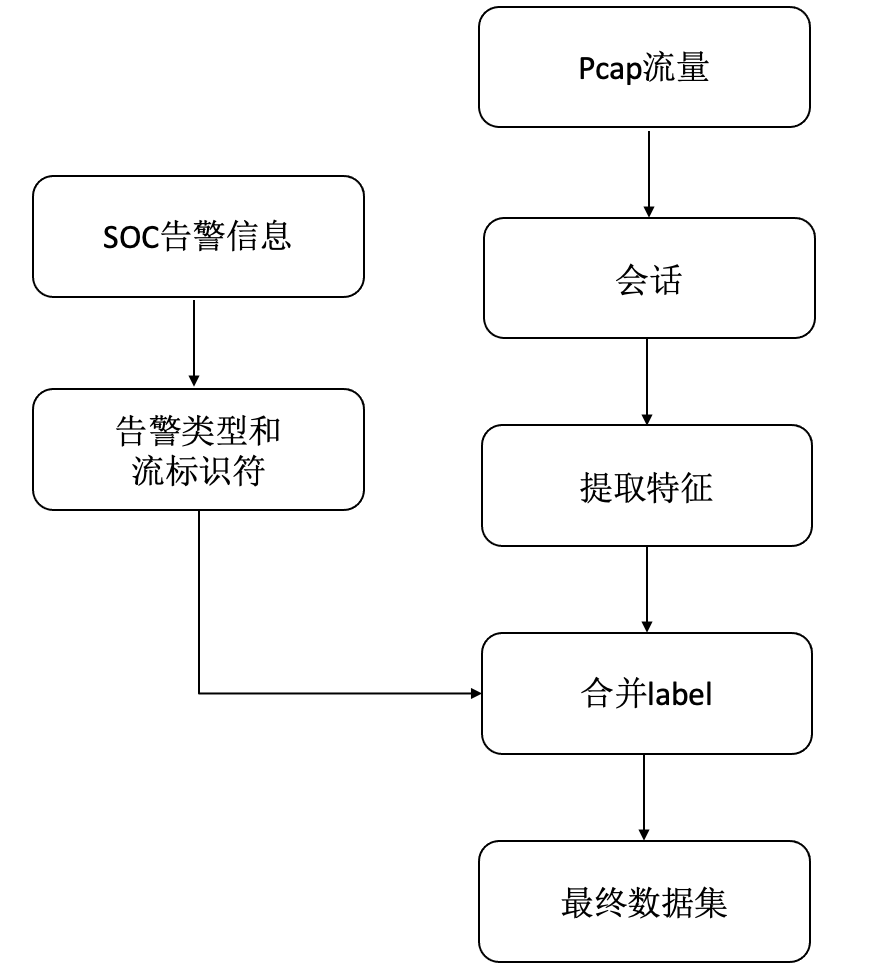
\includegraphics[scale=0.6]{校园网数据集制作流程.png}

    \caption{校园网流量数据集制作流程}
    \label{fig:流量数据集制作流程}
  \end{figure}

在本文的实验中,我们采集了三段共约25小时的数据,第一段从2021年3月19日8点43分采集到2021年3月19日12点08分,持续3.5小时,共420GB大小,用于验证特征提取算法以及经典模型的实验对比,第二段从2021年3月19日13点06分采集到2021年3月20日6点52分,持续18小时,共1100GB大小,用于分析特征关系图的有效性以及训练FG-RNN算法,第三段从2021年3月20日14点26分采集到2021年3月20日18点21分,持续4小时,共350GB大小,用于验证FG-RNN算法的鲁棒性。
% 三段分别持续3.5小时、18小时、4小时,每段大小为420GB、1100GB、350GB。

以上数据为出口网关处的全流量数据,此外我们还利用了安全管理平台(Security Operations Center,SOC)的威胁告警日志,
接下来分别介绍这两类数据。

\subsection{全流量日志数据}
校园网的原始数据为抓包(Packet Capture,pcap)流量,如下图~\ref{fig:wireshark}所示,其中包含每个数据包的详细信息,如五元组、报文头部信息、报文内容等。清华大学校园网共有6个B的地址资源,由于本实验的计算和存储资源的限制,我们只采集了一个B类地址的流量数据,最多可容纳6万台主机,相比于开源数据集采集环境的数十台主机,本数据集规模可谓宏大。

另外,本文对所有用户隐私信息(如IP地址和MAC地址,报文中的明文信息等)都进行了匿名化处理,保证不会泄露用户的任何隐私信息。

\begin{figure}
    \centering
    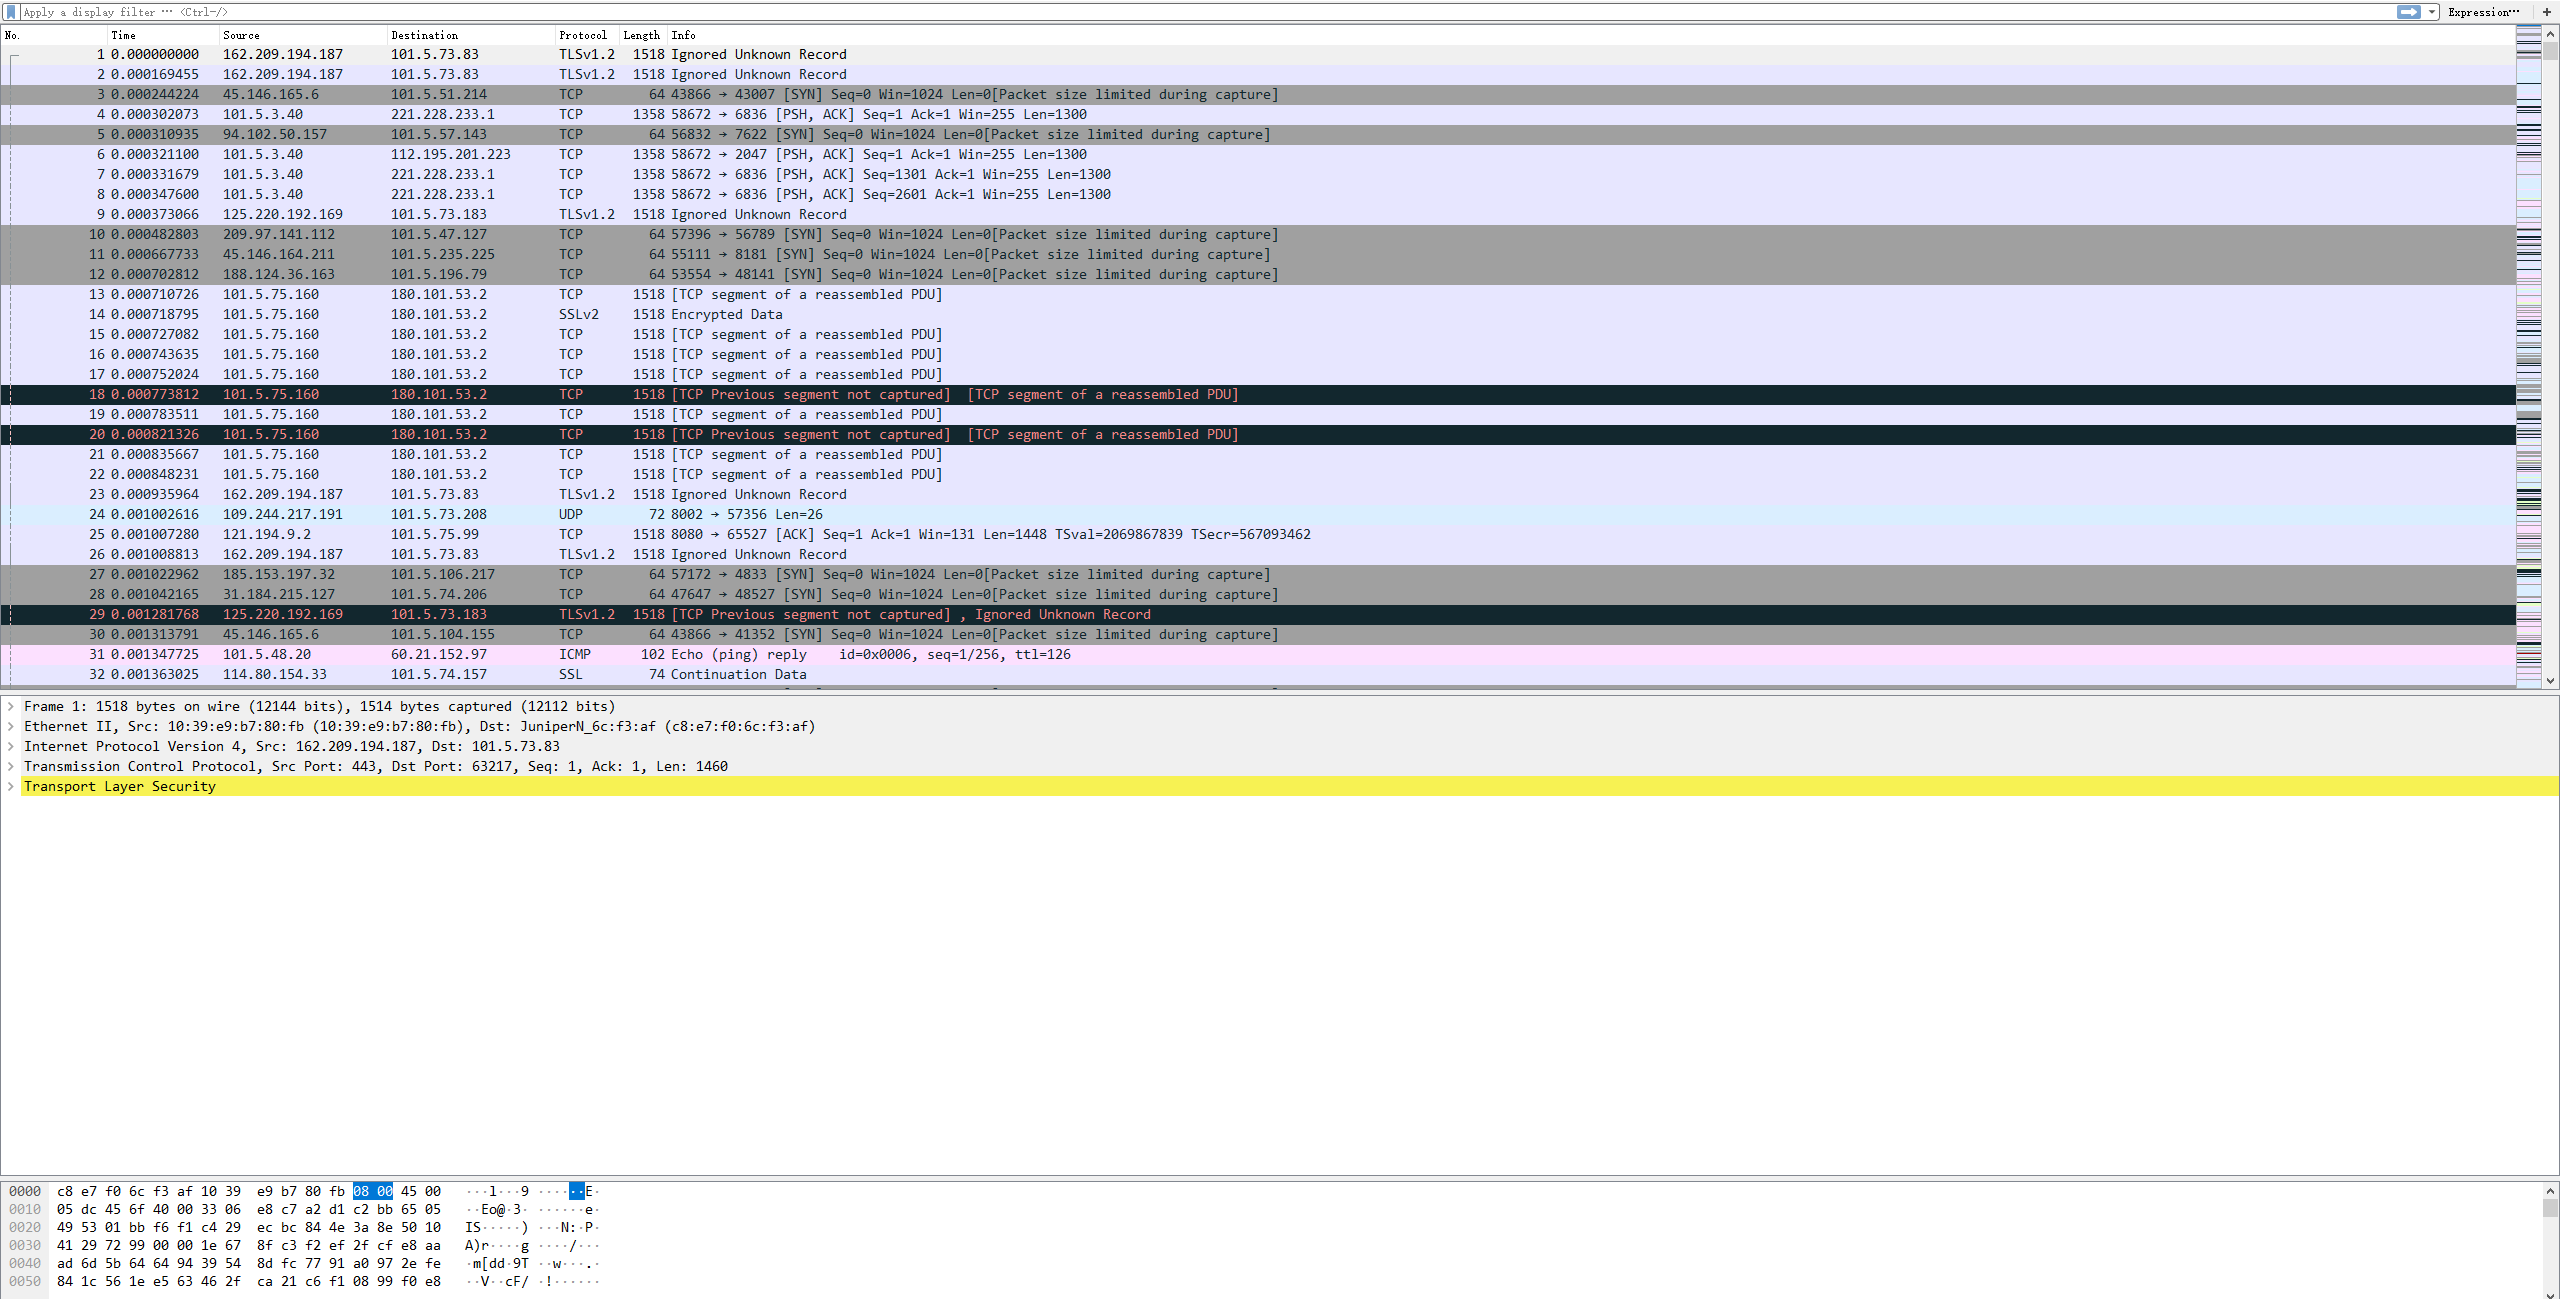
\includegraphics[scale=0.22]{wireshark流量图.png}
    \caption{流量数据示意图}
    \label{fig:wireshark}
  \end{figure}

全流量数据宏观上看具有周期性,例如图\ref{fig:用户流量变化图}表示每秒钟报文数量的变化。但是由于我们是基于每条流的信息进行异常检测,平均每秒钟数百万的报文信息之间大多毫无关联,因此仅需从流的视角对全流量数据进行特征提取。本文采用了CICFlowMeter\footnote{https://github.com/ahlashkari/CICFlowMeter}工具,其大致原理为从pcap文件中依次读取报文(packet),判断当前报文是否属于当前统计的所有流中,若存在则更新该流的统计特征信息,否则创建一条新的流,直至遇到包含FIN标志的报文或者超时。最后将得到的每条流的特征信息依次打印到csv文件中。
%   对于机器学习模型来说,通常
%   不是直接对原始的流量进行检测,而是通过对流量提取特征,得到样本的特征向
%   量后进行检测和分类。


\subsection{威胁告警日志}
我们通过全流量日志得到了特征数据集,但是由于缺乏标注,该数据集无法进行训练以及验证。因此为了得到可进行训练的有效数据集,我们还需要对特征数据集添加标注。我们根据现有的SOC平台得到标注数据,然后进行数据清洗、数据预处理等步骤。图\ref{fig:NOC平台数据样例}为SOC平台的数据样例。
\begin{figure}
    \centering
    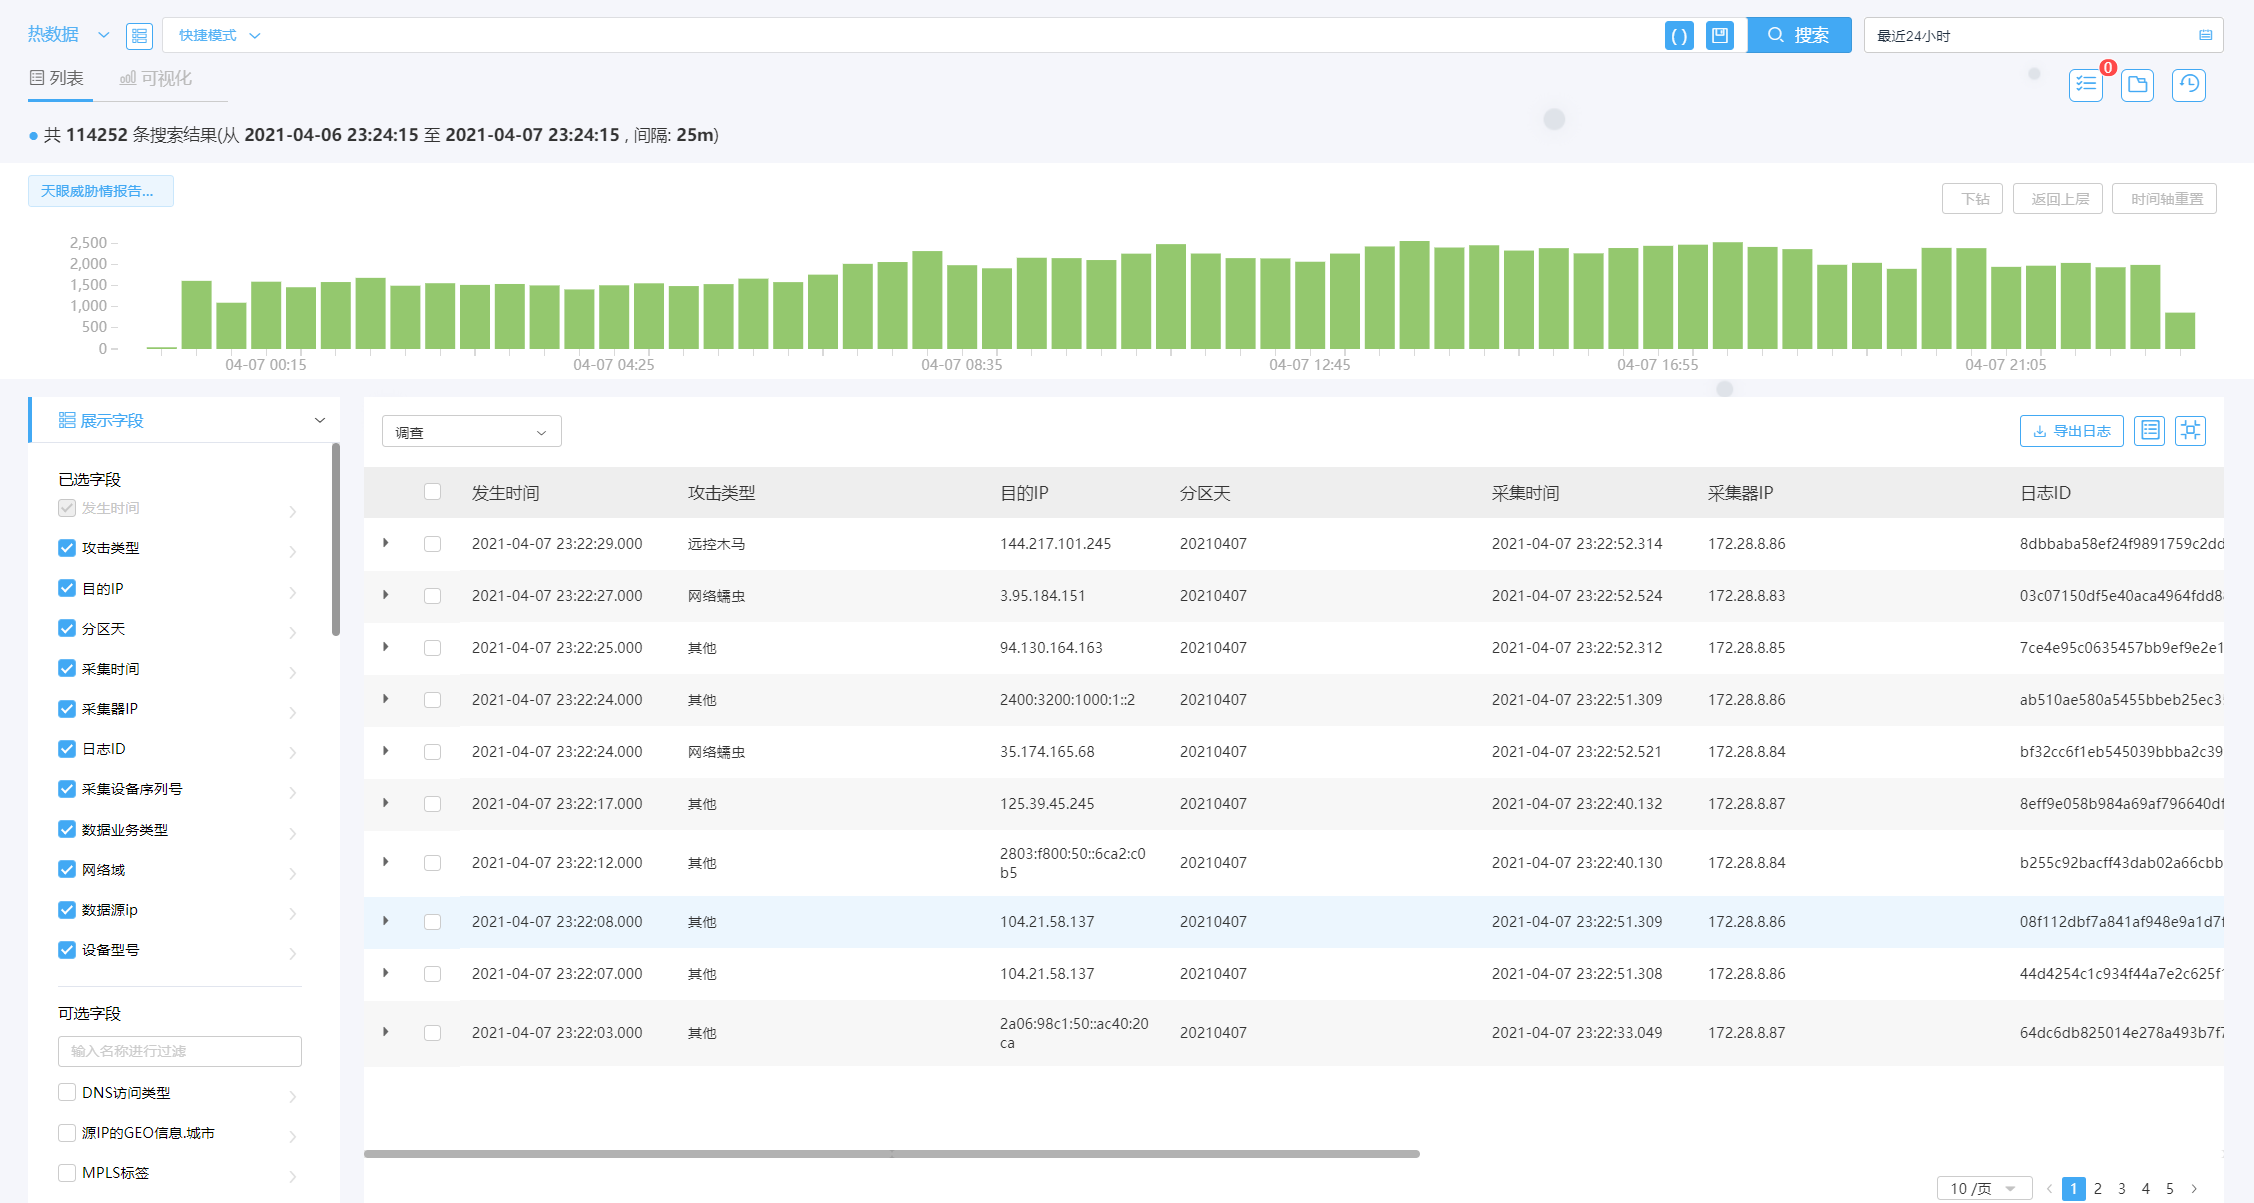
\includegraphics[scale=0.35]{NOC平台.png}
    \caption{SOC平台数据样例}
    \label{fig:NOC平台数据样例}
  \end{figure}


图\ref{fig:告警趋势图}为SOC平台给出的一个月内告警信息的趋势图。从图中可以看出,告警信息大致稳定在每天9000个,存在极端情况。图\ref{fig:告警分布}为告警类型的分布,从中可以看出,远控木马、暴力猜解、后门程序为主要的攻击手段。
\begin{figure}
    \centering
    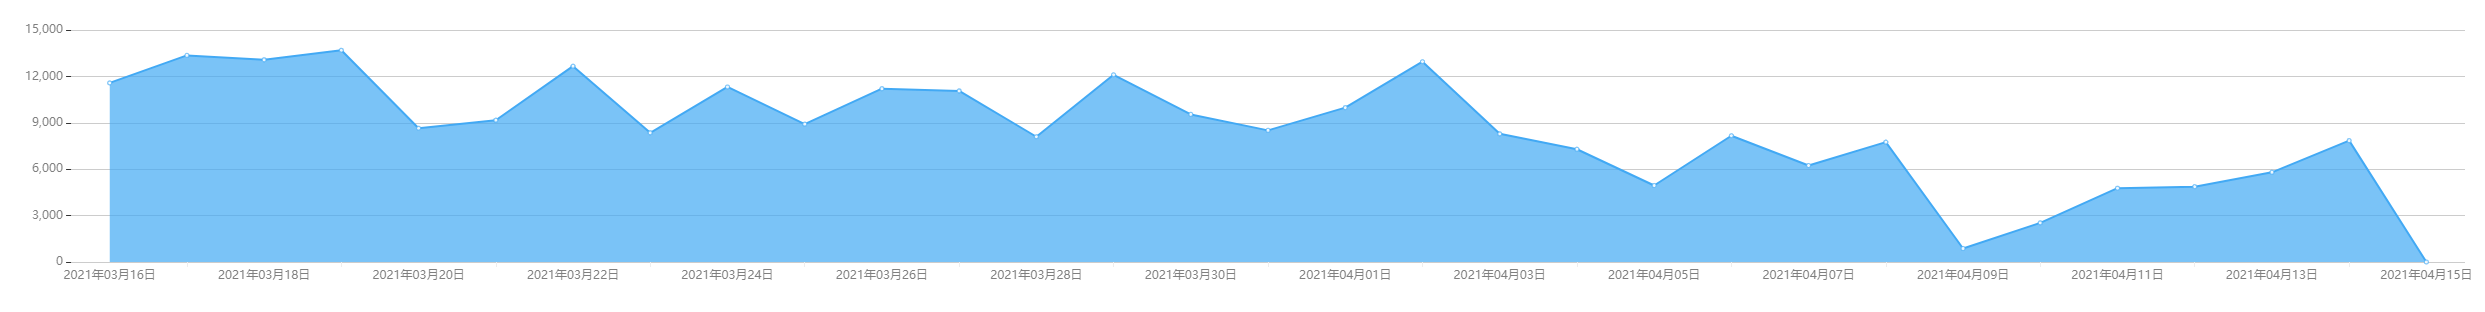
\includegraphics[scale=0.15]{告警趋势图_20214150748.png}
    \caption{告警趋势图}
    \label{fig:告警趋势图}
  \end{figure}
  \begin{figure}
    \centering
    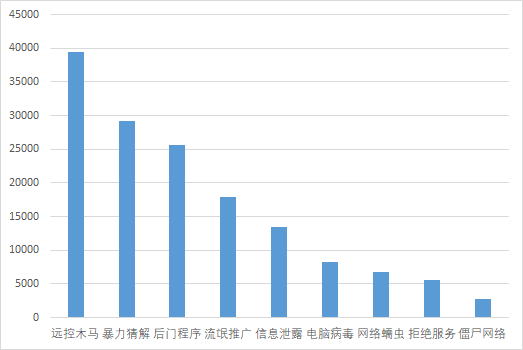
\includegraphics[scale=0.6]{告警分布.png}
    \caption{告警分布}
    \label{fig:告警分布}
  \end{figure}


\section{现有算法在不同数据集的评估}
本文利用sklearn、pytorch等python库分别实现了“逻辑回归(LR)”、“朴素贝叶斯(NB)”、“决策树”(DT)、标准的“循环神经网络”(RNN)、“长短期记忆网络”(LSTM)、“门控循环单元”(GRU)几个模型。

本节分别在以上三个数据集上进行实验,对比了以上6个经典模型,表\ref{不同数据集下实验评估结果}是评估结果,评估指标为正样本的准确率,其中多分类任务的准确率指标为对于每个标签,分别计算precision,然后取不加权平均值。由表中可以看出,在两个开源数据集上,各个算法在二分类任务(即仅需检测是否发生异常)的效果相差不大,在多分类任务(即需要判断异常类型)里,神经网络类的模型效果均要好于基于分类的机器学习模型。这说明针对模拟仿真出的有规律的流量数据,各类算法可以有效地学习出正常流量的基线,而不同类型的异常具有各自的特征,各个算法的能力在学习这些特征的过程中显现出差异。但是这些算法在CAMPUS数据集上表现很差,甚至和随机猜测的效果差不多。说明现有的算法无法应对复杂的清华大学校园网流量环境,需要我们进一步对这些算法进行优化,以适应校园网流量环境。




\begin{table*}[h]
    \small
    \caption{不同数据集下实验评估结果}
    \label{不同数据集下实验评估结果}
    \centering
    \begin{tabular}{c|c|ccc|ccc}
    \toprule
    
     数据集 &  任务  &  
     LR &  NB & DT & RNN & LSTM & GRU  \\
    \midrule
    
    UNSW-NB15 & 二分类 & 84.8 & 79.33 & 78.52 &  80.51 & 62.74 & 68.91  \\ 
    
    & 多分类 &76.73 & 77.96 & 76.82 & 77.98 & 47.11 & 56.30  \\
    
    \midrule
    CICIDS2017 & 二分类 & 68.26 & 67.11 & 65.54 & 70.18 & 65.04 & 68.49  \\
    & 多分类 & 67.01 & 67.37 & 66.41 & 68.31 & 66.16 & 63.18 \\
    \midrule
    CAMPUS & 二分类 & 59.98 & 57.95 & 59.51 & 55.62 & 59.80 & 55.25 \\
    & 多分类 & 56.33 & 57.01 & 57.54 & 53.01 & 56.59 & 59.28 \\
   
     \bottomrule
    
    \end{tabular}
    \end{table*}
